\documentclass{beamer}
\usepackage{algorithm2e}
\usepackage{natbib}
\usepackage{layouts}
\definecolor{vuborange}{rgb}{1.0,0.40,0.0}
\definecolor{darkyellow}{rgb}{1.0,0.79,0.12}
\definecolor{forestgreen}{rgb}{0.13, 0.55, 0.13}
\usetheme{Boadilla}
\usepackage{color,soul}
\usepackage{xcolor}
\usepackage{adjustbox}
\usepackage{amsmath,amssymb}
\usepackage{booktabs}
\usepackage{calc}
\usepackage{subcaption}
\usepackage{graphicx}

\usepackage[bordercolor=white,backgroundcolor=gray!30,linecolor=black,colorinlistoftodos]{todonotes}
\newcommand{\rework}[1]{%
	\todo[color=yellow,inline]{Rework: {#1}}%
}

\usetikzlibrary{shapes.geometric, arrows}

\title{Workshop Explanations: Efficiently Explaining CSPs (with Unsatisfiable Subset Optimization)}
\date{}
\author{\underline{Emilio Gamba}\inst{1} \and  Bart Bogaerts\inst{1} \and   Tias Guns\inst{1,2}}

\newcommand\hlyellow[1]{\hl{ {\sethlcolor{yellow}#1}}}
\newcommand\hlgreen[1]{\sethlcolor{green}\hl{#1}}

\newcommand\m[1]{\ensuremath{\mathcal{#1}}\xspace}
\renewcommand\emph[1]{{\color{vuborange}#1}}

\renewcommand{\thealgocf}{}

\newtheorem{exsudoku}{ExampleSudoku}
\newtheorem{examplesudoku}[exsudoku]{Example (Sudoku)}

\makeatletter
\renewcommand{\@algocf@capt@plain}{above}% formerly {bottom}
\setbeamertemplate{footline}
{
	\leavevmode%
	\hbox{%
		\begin{beamercolorbox}[wd=.15\paperwidth,ht=2.25ex,dp=1ex,center]{author in head/foot}%
			\usebeamerfont{author in head/foot}Emilio Gamba
		\end{beamercolorbox}%
		\begin{beamercolorbox}[wd=.55\paperwidth,ht=2.25ex,dp=1ex,center]{title in head/foot}%
			\usebeamerfont{title in head/foot}Efficiently Explaining CSPs with Unsatisfiable Subset Optimization
		\end{beamercolorbox}%
		\begin{beamercolorbox}[wd=.3\paperwidth,ht=2.25ex,dp=1ex,right]{date in head/foot}%
			\usebeamerfont{date in head/foot}Leuven-explanations 2022\hspace*{1em}
			\insertframenumber{} / \inserttotalframenumber\hspace*{2ex} 
	\end{beamercolorbox}}%
	\vskip0pt%
}
\makeatother

\usepackage{enumitem}
\newlist{RQ}{enumerate}{1}
\setlist[RQ]{label=\bfseries{}RQ\arabic*:}
\newlist{WP}{enumerate}{1}
\setlist[WP]{label=\bfseries{}RQ\arabic*:}

\begin{document}
	
	\begin{frame}
		\maketitle
		\begin{minipage}{0.20\textwidth}
			\begin{flushleft}
				
\includegraphics[width=\textwidth]{template_vub/VUB-AI_RGB-1-800x223}
			\end{flushleft}
		\end{minipage}		\hfill
	\begin{minipage}{0.10\textwidth}
	
	
\includegraphics[width=\textwidth]{figures/DTAI_Logo_2}
\end{minipage}
\hfill
	\begin{minipage}{0.15\textwidth}
		
\includegraphics[width=0.7\textwidth]{figures/datalab_400x400.jpg}
	\end{minipage}
	\end{frame}
	
	\section{Motivation}
	\begin{frame}{I'm stuck... What should I do now ?}
		\begin{minipage}{0.4\textwidth}
			\only<1>{
	\begin{figure}[H]
		\centering
		\includegraphics[width=0.9\textwidth]{figures/sudoku_steps/sudoku-step1}
	\end{figure}
}
\only<2>{
	\begin{figure}[H]
		\centering
		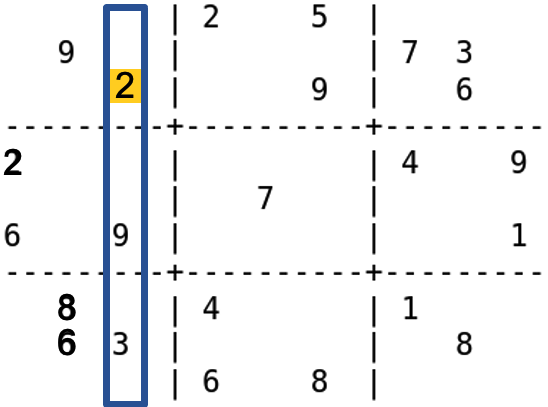
\includegraphics[width=0.9\textwidth]{figures/sudoku_steps/sudoku-step2}
	\end{figure}
}
\only<3>{
	\begin{figure}[H]
		\centering
		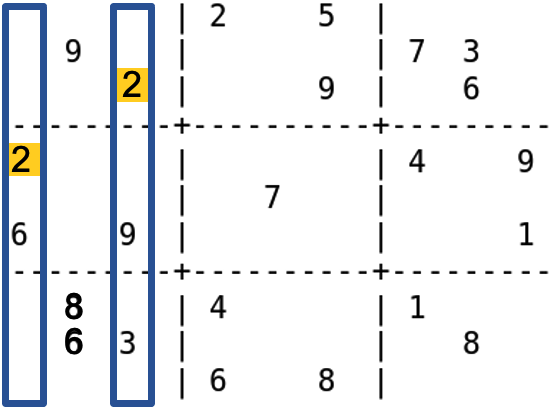
\includegraphics[width=0.9\textwidth]{figures/sudoku_steps/sudoku-step3}
	\end{figure}
}
\only<4>{
	\begin{figure}[H]
		\centering
		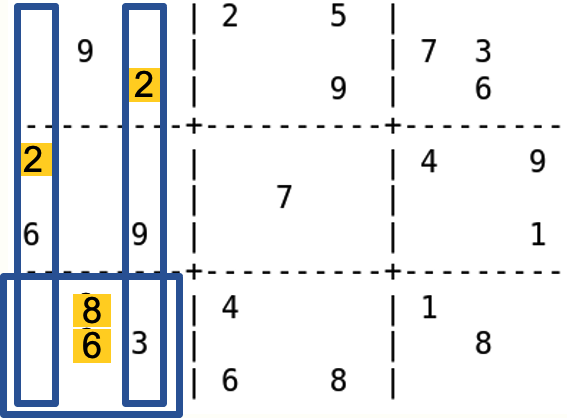
\includegraphics[width=0.9\textwidth]{figures/sudoku_steps/sudoku-step4}
	\end{figure}
}
\only<5->{
	\begin{figure}[H]
		\centering
		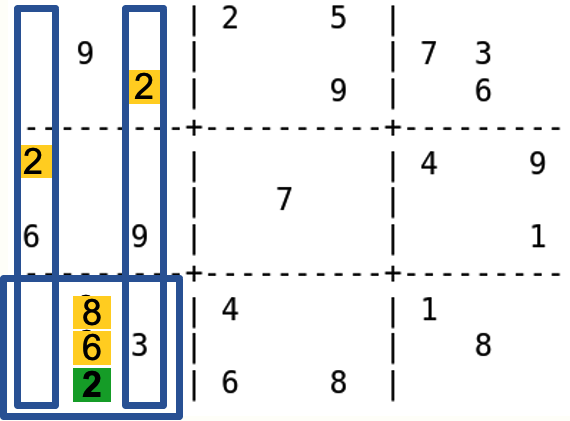
\includegraphics[width=0.9\textwidth]{figures/sudoku_steps/sudoku-step5}
	\end{figure}
}

\begin{itemize}
	\item[{
\includegraphics[width=15pt]{figures/explanation_steps/explanation_S_full}}] Constraints 
	\item[{
\includegraphics[width=15pt]{figures/explanation_steps/explanation_E_full}}] Facts, i.e. given sudoku numbers
	\item[{
\includegraphics[width=15pt]{figures/explanation_steps/explanation_N}}] A newly derived fact
\end{itemize}
\end{minipage}\hfill
\begin{minipage}{0.55\textwidth}
\only<6->{

	\begin{examplesudoku}
		
		{\Large $\mathtt{\mathbf{OCUS}}($}{\large 
\includegraphics[width=10pt]{figures/explanation_steps/explanation_S_full} $\&$
			 {
\includegraphics[width=10pt]{figures/explanation_steps/explanation_E_full}} $\& \lnot$ {
\includegraphics[width=10pt]{figures/explanation_steps/explanation_N}} $, f , p)$ } \\ 
		\vspace{0.5cm}
				 $\{$\colorbox{white}{$\mathtt{alldifferent-COL_1},$} \colorbox{darkyellow}{$V_{(4, 1)}  = 2$},\\
$\{$\colorbox{white}{$\mathtt{alldifferent-COL_3},$} \colorbox{darkyellow}{$ V_{(3, 3)}  = 2$}, \\  
$\{$\colorbox{white}{$\mathtt{alldifferent-BLOCK_{(3,3)}}$},\\  
\colorbox{darkyellow}{$V_{(7, 2)}  = 8$}, \colorbox{darkyellow}{$V_{(8, 2)}  = 6$}, 	 \colorbox{forestgreen}{$V_{(9, 2)}  \neq 2$}$\} $
		\begin{center}
			\textbf{or}
		\end{center}
				 $\{$\colorbox{white}{$\mathtt{alldifferent-COL_1},$} \colorbox{darkyellow}{$V_{(4, 1)}  = 2$},\\
		$\{$\colorbox{white}{$\mathtt{alldifferent-COL_3},$} \colorbox{darkyellow}{$ V_{(3, 3)}  = 2$}, \\  
		$\{$\colorbox{white}{$\mathtt{alldifferent-BLOCK_{(3,3)}}$},\\  
		\colorbox{darkyellow}{$V_{(7, 2)}  \neq 2$}, \colorbox{darkyellow}{$V_{(8, 2)}  \neq 2$},  \colorbox{forestgreen}{$V_{(9, 2)}  \neq 2$}$\} $

\end{examplesudoku}
}
\end{minipage}
\end{frame}

	\begin{frame}
	\frametitle{What is a \emph{good} explanation ?}
	\begin{minipage}{0.25\textwidth}
		\includegraphics[width=\textwidth]{figures/sudoku_sequence/sudoku-step1.png}
	\end{minipage} \pause $\rightarrow$
	\begin{minipage}{0.28\textwidth}
		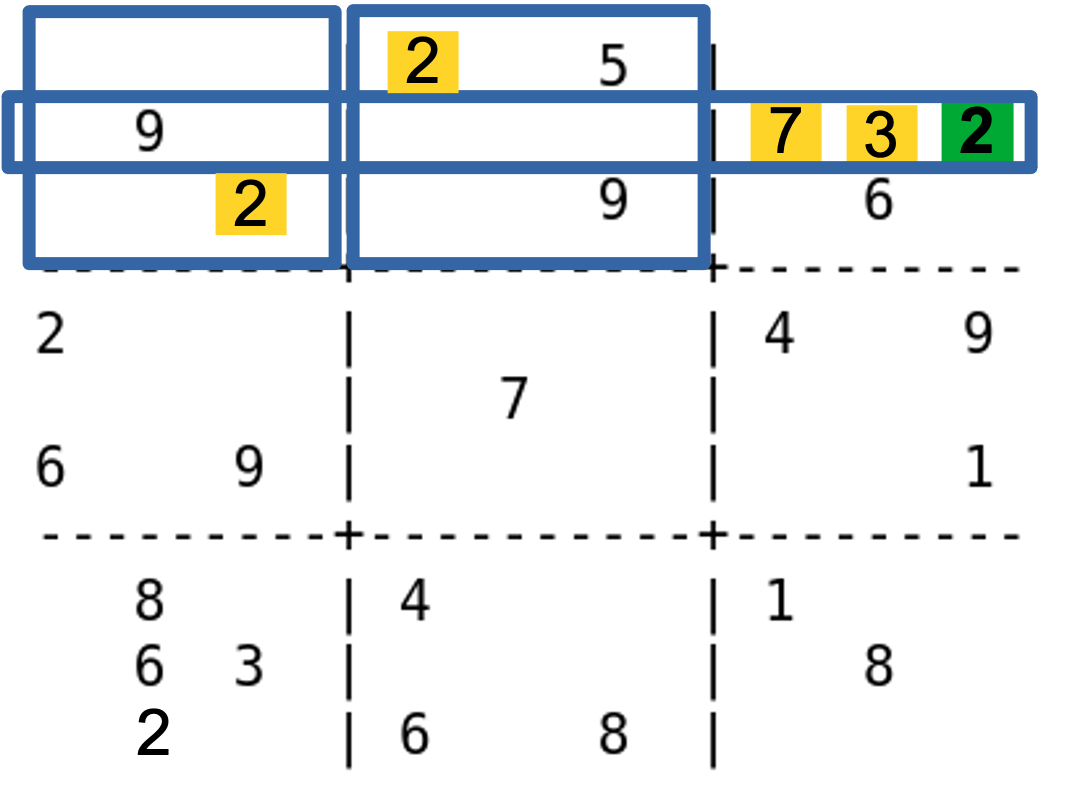
\includegraphics[width=\textwidth]{figures/sudoku_sequence/sudoku-step2}
	\end{minipage}\hfill \pause
	or \hfill
	\begin{minipage}{0.30\textwidth}
		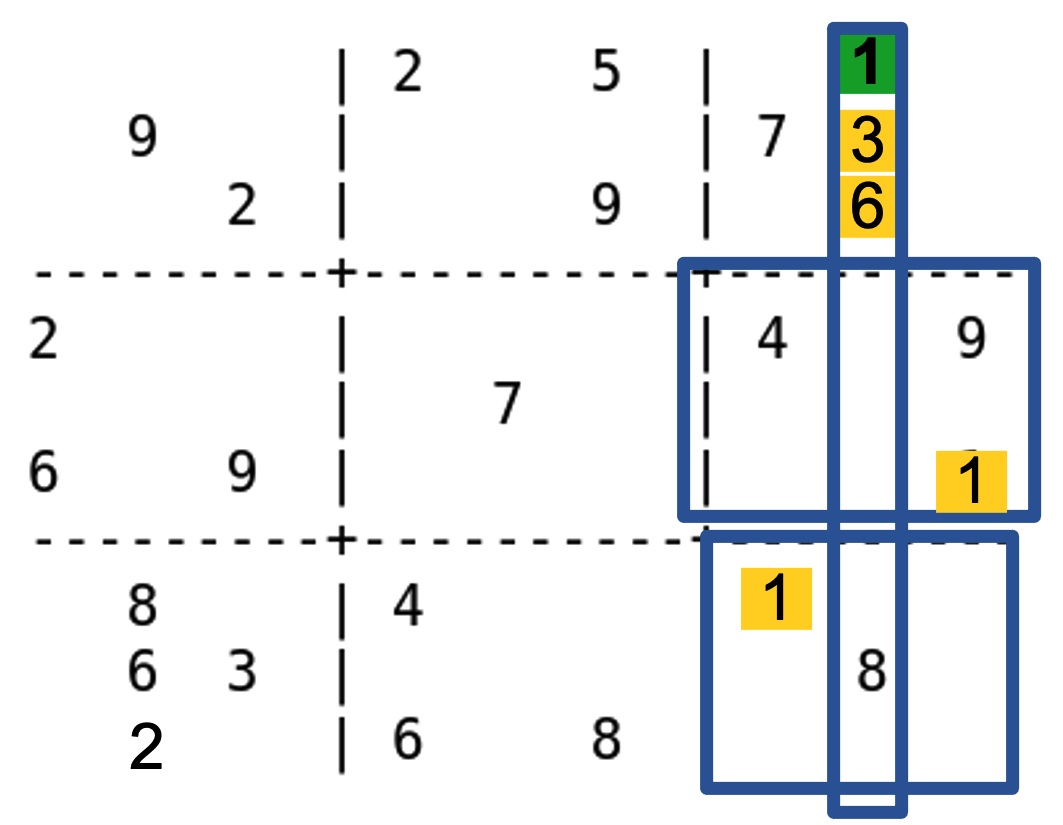
\includegraphics[width=\textwidth]{figures/sudoku_sequence/sudoku-step3bis}
	\end{minipage}\pause\vfill
\begin{itemize}
\item Which constraints should I use ?\pause
\item Which digit should I explain first ?\pause
\item Can I build a cost-function $f$ that can help me characterize good explanations ?
\end{itemize}
\end{frame}	


\begin{frame}
	\begin{minipage}{0.28\textwidth}
		\includegraphics[width=\textwidth]{figures/sudoku_sequence/sudoku-step1}
	\end{minipage}\hfill\pause
	\begin{minipage}{0.045\textwidth}
		\begin{center}
			$\rightarrow$
		\end{center}
	\end{minipage}\hfill
	\begin{minipage}{0.28\textwidth}
		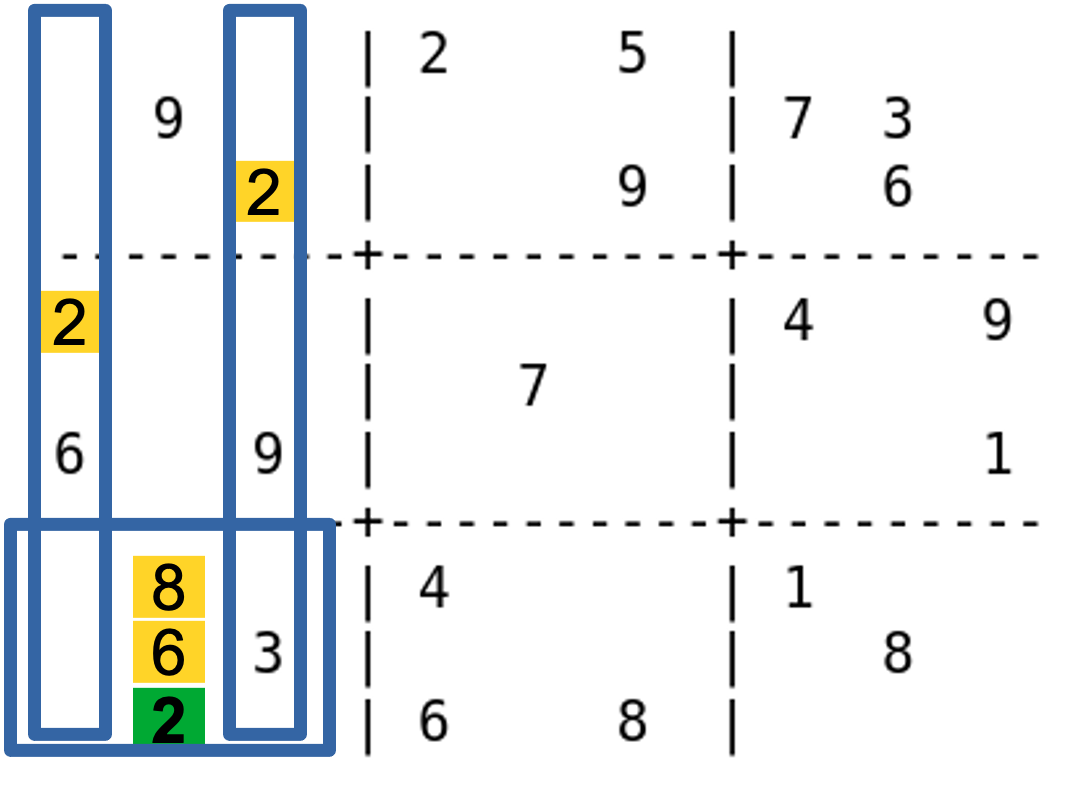
\includegraphics[width=\textwidth]{figures/sudoku_steps/sudoku3}
	\end{minipage}\hfill
	\begin{minipage}{0.045\textwidth}
		\begin{center}
			$\rightarrow$
		\end{center}
	\end{minipage}\hfill
	\begin{minipage}{0.28\textwidth}
		\begin{center}
			$\dots$
		\end{center}
	\end{minipage}\\\vfill
\only<0->{
	\begin{center}
		What is a \emph{sequence} of explanations ? 
	\end{center}
}\vfill
 \pause
	\begin{minipage}{0.28\textwidth}
		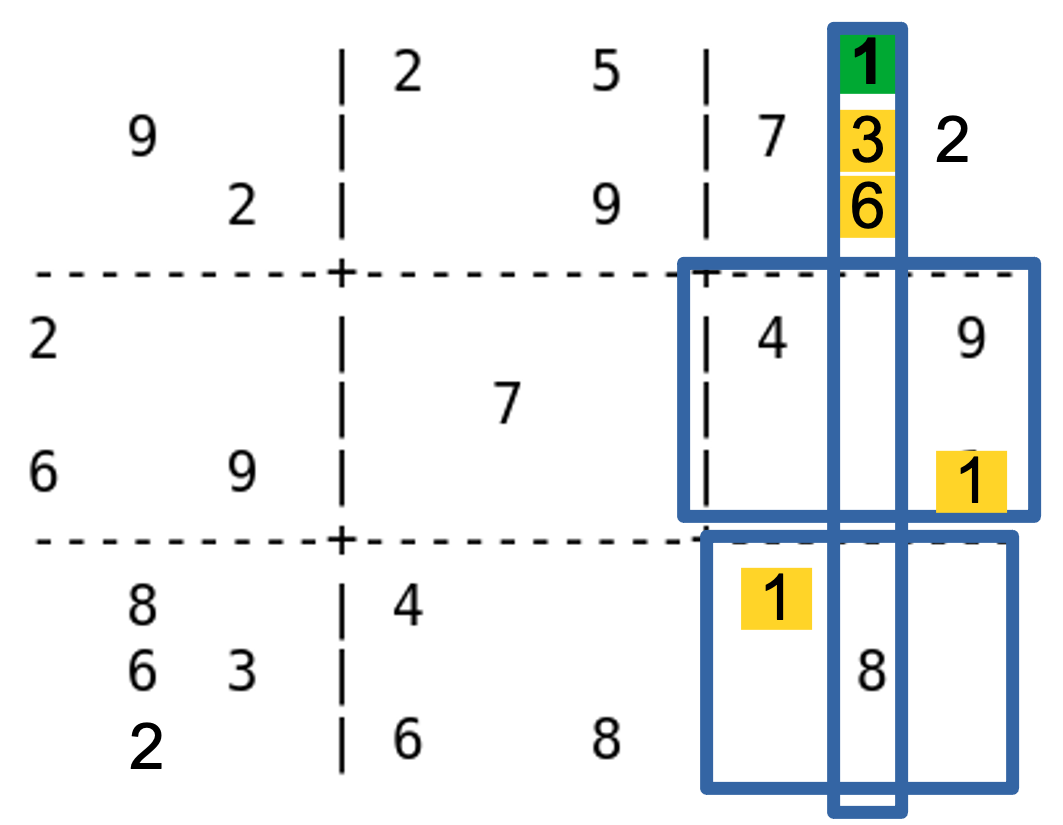
\includegraphics[width=\textwidth]{figures/sudoku_sequence/sudoku-step3}
	\end{minipage}
	\hfill
	\begin{minipage}{0.43\textwidth}
		\begin{center}
			$\rightarrow$ \hspace{0.5cm}\dots \hspace{0.5cm}$\rightarrow$
		\end{center}
	\end{minipage}\hfill\pause
	\begin{minipage}{0.28\textwidth}
		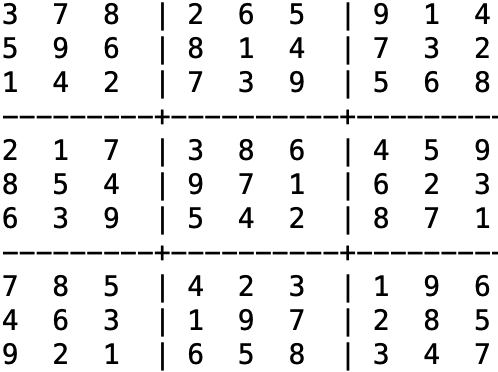
\includegraphics[width=\textwidth]{figures/sudoku_sequence/sudoku-stepn}
	\end{minipage}
\end{frame}

\begin{frame}

	\begin{minipage}{0.28\textwidth}
		\includegraphics[width=\textwidth]{figures/sudoku_sequence/sudoku-step1}
	\end{minipage}\hfill
	\begin{minipage}{0.045\textwidth}
		\begin{center}
			$\rightarrow$
		\end{center}
	\end{minipage}\hfill
	\begin{minipage}{0.28\textwidth}
		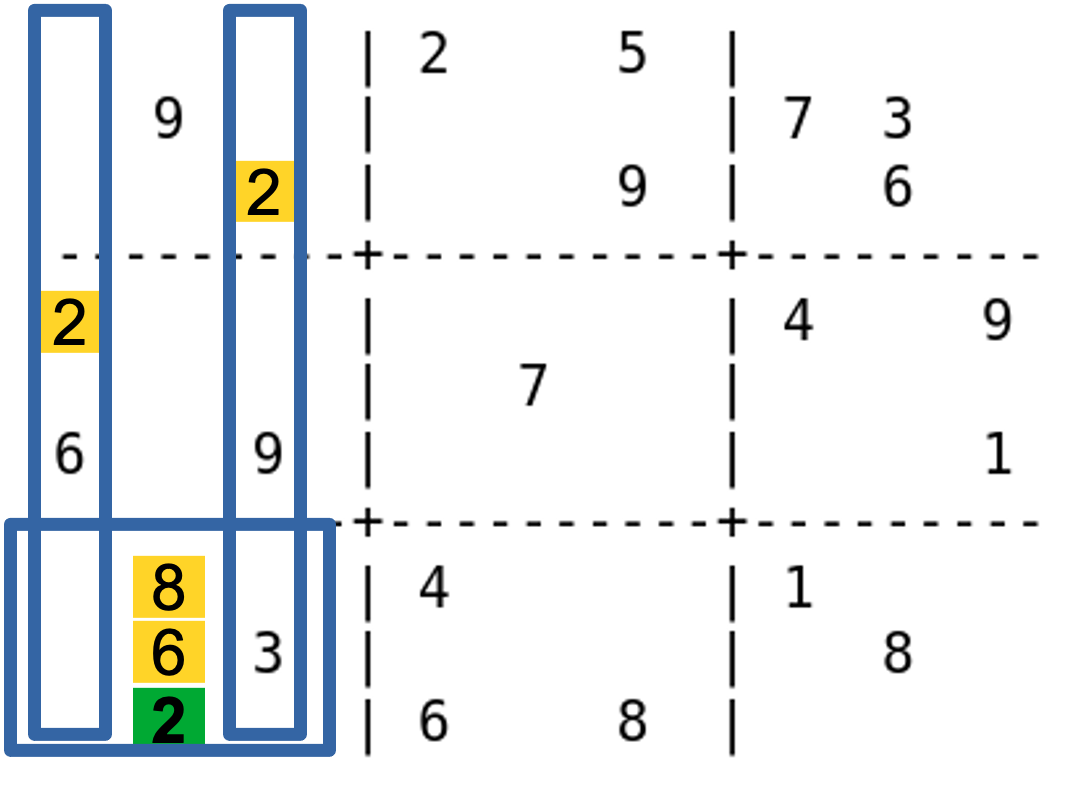
\includegraphics[width=\textwidth]{figures/sudoku_steps/sudoku3}
	\end{minipage}\hfill
	\begin{minipage}{0.045\textwidth}
		\begin{center}
			$\rightarrow$
		\end{center}
	\end{minipage}\hfill
	\begin{minipage}{0.28\textwidth}
		\begin{center}
			$\dots$
		\end{center}
	\end{minipage}\\\vfill
\begin{center}
What is a \textbf{\emph{GOOD}} sequence of explanations ? 
\end{center}
 \vfill
	\begin{minipage}{0.28\textwidth}
		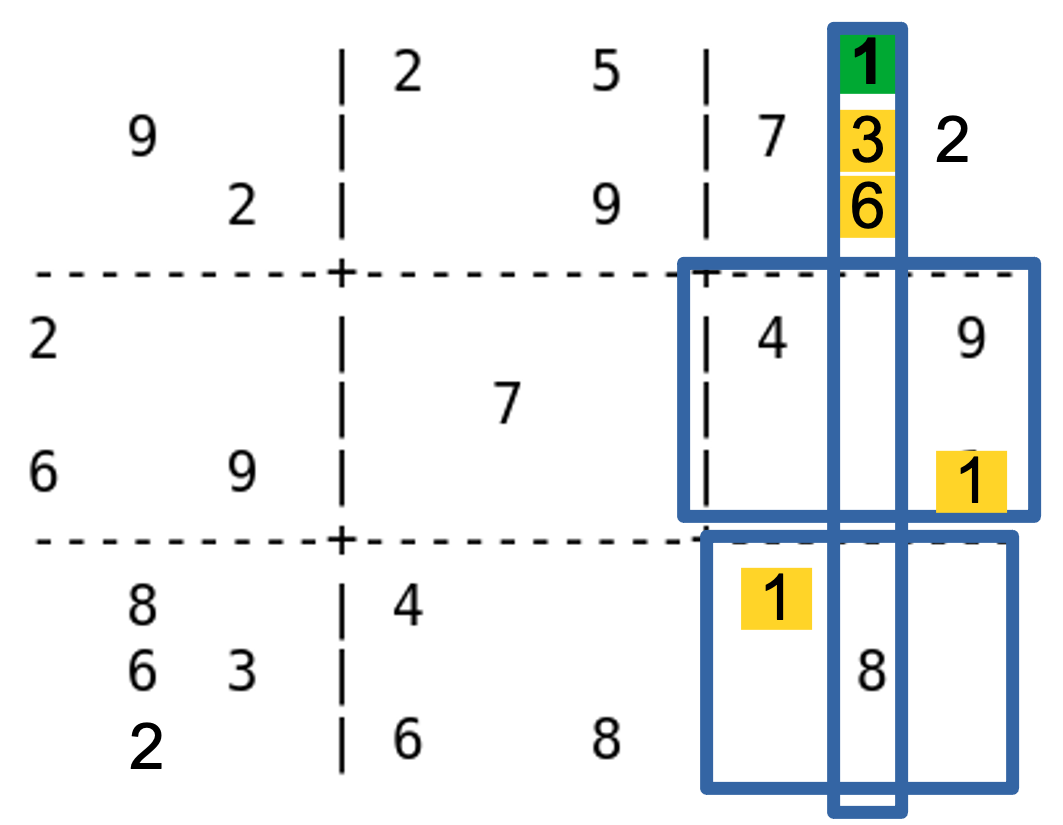
\includegraphics[width=\textwidth]{figures/sudoku_sequence/sudoku-step3}
	\end{minipage}
	\hfill
	\begin{minipage}{0.43\textwidth}
		\begin{center}
			$\rightarrow$ \hspace{0.5cm}\dots \hspace{0.5cm}$\rightarrow$
		\end{center}
	\end{minipage}\hfill
	\begin{minipage}{0.28\textwidth}
		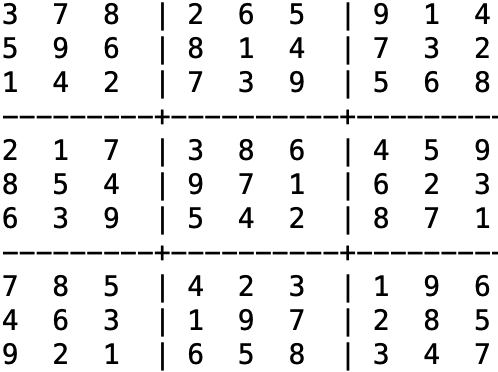
\includegraphics[width=\textwidth]{figures/sudoku_sequence/sudoku-stepn}
	\end{minipage}
\end{frame}
				\begin{frame}
				\textbf{RQ1 - Which are the features of an explanation?}
				\begin{itemize}
					\item \# facts in a step, domain-specific vs domain-independent information, constraints decomposition , ...
					\item How do we encode the features of a good explanation in the cost function?
%					\item What are the limitations of the current state-of-the-art for effectively computing explanations using OCUSs?
				\end{itemize}
				\textbf{RQ2 - How to reconcile auto-generated sequences of explanations with human-generated solving traces?} 
				\begin{itemize}
					\item How do we capture the preferences of a user based on the features we have extracted for a good explanation?
					\item What are the global metrics  for characterizing the quality of an explanation sequence?
				\end{itemize}

				\end{frame}

			\begin{frame}
				\textbf{RQ3 - Is it always possible to generate a meaningful nested explanation sequence at a lower abstraction level?}
				\begin{itemize}
					\item AIJOURNAL-counterfactual explanations: Nested explanations $\rightarrow$ abstraction level lower
					\item All-domain reductions needed 
				\end{itemize}
			Observations:
			\begin{itemize}
%				\item 
				\item {\color{red} Here we are extending the explanation language for explaining when we go one abstraction level lower and use the domain reductions}
				\item {\color{red} We can nest as much as we want !}
			\end{itemize}
				\end{frame}
			
		\begin{frame}[allowframebreaks]
			\frametitle{References}
			\bibliographystyle{named}
			\bibliography{refs,references}
		\end{frame}
		
		
		
		
		
	\end{document}
	
	
	
	
	
	
	
	
	
